\documentclass{article}
\newcommand{\vk}[1]{{\color{blue}{#1}}}

\usepackage{exercise}
\usepackage[obeyspaces]{url}
\usepackage[dvipsnames]{xcolor}
\usepackage{graphicx}
\usepackage{listings}
\usepackage[scaled]{helvet}
\usepackage{amsmath,amssymb,amsfonts,mathtools,cancel}

% typeset in helvetica
\renewcommand*\familydefault{\sfdefault}


% QE stuff
\def\qe{{\sc Quantum ESPRESSO}}
\def\pwx{\texttt{pw.x}}
\def\cpx{\texttt{cp.x}}
\def\phx{\texttt{ph.x}}
\def\nebx{\texttt{neb.x}}
\def\configure{\texttt{configure}}
\def\PWscf{\texttt{PWscf }}
\def\PHonon{\texttt{PHonon}}
\def\CP{\texttt{CP}}
\def\PostProc{\texttt{PostProc}}
\def\NEB{\texttt{PWneb}} % to be decided
\def\make{\texttt{make}}
%%%%%%%%%%%%%%%%%%%%%%%%

\def\ipi{i-PI}
\newcommand{\hints}[1]{\emph{Hints: #1}}
\newcommand{\lstinxml}{\lstinline[language=XML]}
\newcommand{\lstinbash}{\lstinline[language=Bash]}
\usepackage[space=true]{accsupp}

\newcommand{\pdfactualhex}[3]{\newcommand{#1}{%
\BeginAccSupp{method=hex,ActualText=#2}#3\EndAccSupp{}}}

% PASTABLE lstlisting code
\pdfactualhex{\pdfactualdspace}{2020}{\textperiodcentered\textperiodcentered}
\pdfactualhex{\pdfactualsquote}{27}{'}
\pdfactualhex{\pdfactualbtick}{60}{`}

\lstset{tabsize=4,basicstyle=\ttfamily,breaklines=true,columns=flexible,emptylines=10000}
\lstset{literate={'}{\pdfactualsquote}1
                 {`}{\pdfactualbtick}1
                 {\ \ }{\pdfactualdspace}2
}

\lstset{
    basicstyle=\ttfamily,
    keywordstyle=\color{BrickRed},
    commentstyle=\color{Gray},
    stringstyle=\color{black},
    emphstyle=\color{RedOrange},
    columns=flexible,
    showstringspaces=false,
    xleftmargin=1em,
    deletekeywords={bin,all}
}


\lstdefinelanguage{Bash}
{
   alsodigit={-,.},
   morekeywords={ cp2k.popt, lmp_ubuntu, i-pi, vmd, for, done, python, mpirun, touch, tail, trajworks, autocorr, awk, i-pi-mergebeadspdb, grep, head, cp, cd, cat, ls, pwd, bash, sed, mkdir, vi, sh}
   %morecomment=[s][\color{orange}]{#}{\}
}

%\lstdefinelanguage{Python}
%{
%    morecomment=[s][\color{orange}]{#}{\}
%}


\lstdefinelanguage{XML}
{
  morestring=[b][\color{RedOrange}]",
%  morestring=[s]{>}{<},
  morecomment=[s]{<?}{?>},
  morecomment=[s][\color{orange}]{<!--}{-->},
  identifierstyle=\color{BlueViolet},
  keywordstyle=\color{ForestGreen},
  stringstyle=\color{RedOrange},
%  tagstyle=\color{Blue},
  morekeywords={xmlns,version,type, mode, units, forcefield, filename, stride, overwrite, nbeads,prefix}% list your attributes here
}

\lstdefinestyle{XML}
{
\tagstyle=\color{Blue}
}

\title{Advanced Path Integral Methods in a \\ Simulation of Water Across 
  its Phase Diagram}
\author{Michele Ceriotti}
\date{June 2018}

\begin{document}

\maketitle

% INTRO
In this set of exercises we will perform
simulations of room-temperature liquid water,
using a simple empirical forcefield model based
on TIP4P-like point charges~\cite{habe+09jcp}. 
We will start from quickly checking the convergence of 
standard path integral molecular
dynamics, and then use this 
example to test a number of 
advanced PI features. For the sake of 
speed of execution, we will use a very
small (32 molecules) simulation box. 
However, if you have more time to carry
out the exercise, you can modify
the input to use the initial
configurations in \url{data/water-216.pdb}.
You should be able to complete at least the first three
exercises in a couple of hours. \hints{Do not wait for the full
simulations to be complete: as soon as you have collected
enough statistics to understand what's going on and to 
compare with previous runs, you should move on to the next
exercise.}

\begin{Exercise}[label={basic},title={A PIMD simulation of liquid water}]

\Question 
Look at the \ipi{} input file in \url{ex-1/base.xml}. Observe the 
properties and trajectory files that are specified in the \lstinxml$<output></output>$ section. 
Make sure it is clear what each part 
of the input does. For this example
we will use the PILE-G thermostat\cite{ceri+11jcp} and 
constant-temperature sampling. We will 
initially perform a reference molecular dynamics run, with $P=1$. 

\begin{lstlisting}[language=bash]
$ cd ex-1 
$ i-pi base.xml &> log.ipi &
$ lmp_serial < in.water &> log.lammps & 
\end{lstlisting}%$

\Question
Modify the input so that you'll run with
$P=6$ beads, by changing the \lstinxml$nbeads$ option of the \lstinxml$<initialize>$ field. 
It is advisable to make these changes on a copy of the  \url{ex-1/base.xml} input file.
You may also want to adjust \lstinxml$prefix$ so that it indicates the new number of beads (e.g. \lstinxml$prefix="base_p-6"$).
Repeat with $P=32$. \hints{Simulations may take some time to complete so you might want 
to launch all of them and continue with the following exercises. 
In order to run multiple \ipi{} 
simulations simultaneously you should also change the name of the UNIX-domain socket 
-- that is the \lstinxml$<address>$ field 
in the input of \ipi{}, and the corresponding
label in the \lstinbash$fix_ipi$ command 
in the input of LAMMPS.}

\Question
Analyze the outcomes of the simulations and check for convergence. 
You can quickly compute averages for thermodynamic quantities from the command
line using the \url{autocorr} code, e.g. for the potential energy. \hints{\url{autocorr}
will also compute error estimates that take into account the autocorrelation time for the
observable. With short trajectories, this tends to be significantly under-estimated.
Note also that we are discarding a short part of the trajectory for equilibration - in a
production calculation you should carefully check equilibration and discard a part of the
trajectory accordingly.}

\begin{lstlisting}[language=bash]
$ tail -n +50 base_p-1.out | awk '{print $6}' | \
       autocorr -maxlag 100 | head
\end{lstlisting}

\Question
Have a look at the trajectories with the VMD software 
\hints{You can launch VMD from the command line with e.g. 
\lstinbash$vmd base_p-1.pos_0.pdb$}. 
You can load all of the ring polymer beads as separate molecules to visualize the
spread of the ring polymer.
\begin{lstlisting}[language=bash]
$ vmd -m base_p-32.pos_*.pdb 
\end{lstlisting}%$
and you can also use some of the \ipi{} post-processing tools to visualize
the connections within the ring polymer. \hints{Note that you have to load 
the file from the TCL prompt in VMD to disable automatic bond detection.}
\begin{lstlisting}[language=bash]
$ i-pi-mergebeadspdb base_p-32 > base_p-32_merged.pdb
$ vmd
vmd > mol new base_p-32_merged.pdb type pdb autobonds 0
\end{lstlisting}
You can see clearly the different spread of the ring polymers of H and O atoms.

\Question
Compute radial distribution functions for different simulations. You
can use any tool of your liking, but we suggest the \url{trajworks} 
post-processing tool that is part of the \url{toolbox} library.
For instance, for one of the replicas in the 32-beads run,
\begin{lstlisting}[language=bash]
$ trajworks -ipdb -vbox -fstart 10 -gr -gr1 O -gr2 O \
        -grmax 5 -grbins 250 -hwin triangle -hwinfac 2 \
         < base_p-32.pos_00.pdb > gOO.dat
\end{lstlisting}%$
Also compute the O--H radial distribution function.

\end{Exercise}

\begin{Exercise}[label={piglet},title={Colored-noise thermostatting}]

Move to the \url{ex-2/} folder. Here we will try to reduce the number of 
path integral replicas needed to converge a PIMD simulation by using 
a colored-noise thermostat, designed to selectively enhance fluctuations 
of high-frequency modes, so as to match the quantum predictions~\cite{ceri-mano12prl}.

\Question 
Look at the input file. The only significant difference relative to
Exercise~\ref{basic} is the change in the \lstinxml$<thermostat>$ section. 
The matrix elements that are included in this section determine the behavior
of the colored-noise dynamics, and have been fitted to give the correct
quantum fluctuations in the harmonic limit. Parameters that are suitable for
a broad range of conditions can be obtained from the on-line repository
\url{http://gle4md.org/index.html?page=matrix} -- familiarize
yourself with the interface.

\ExeText
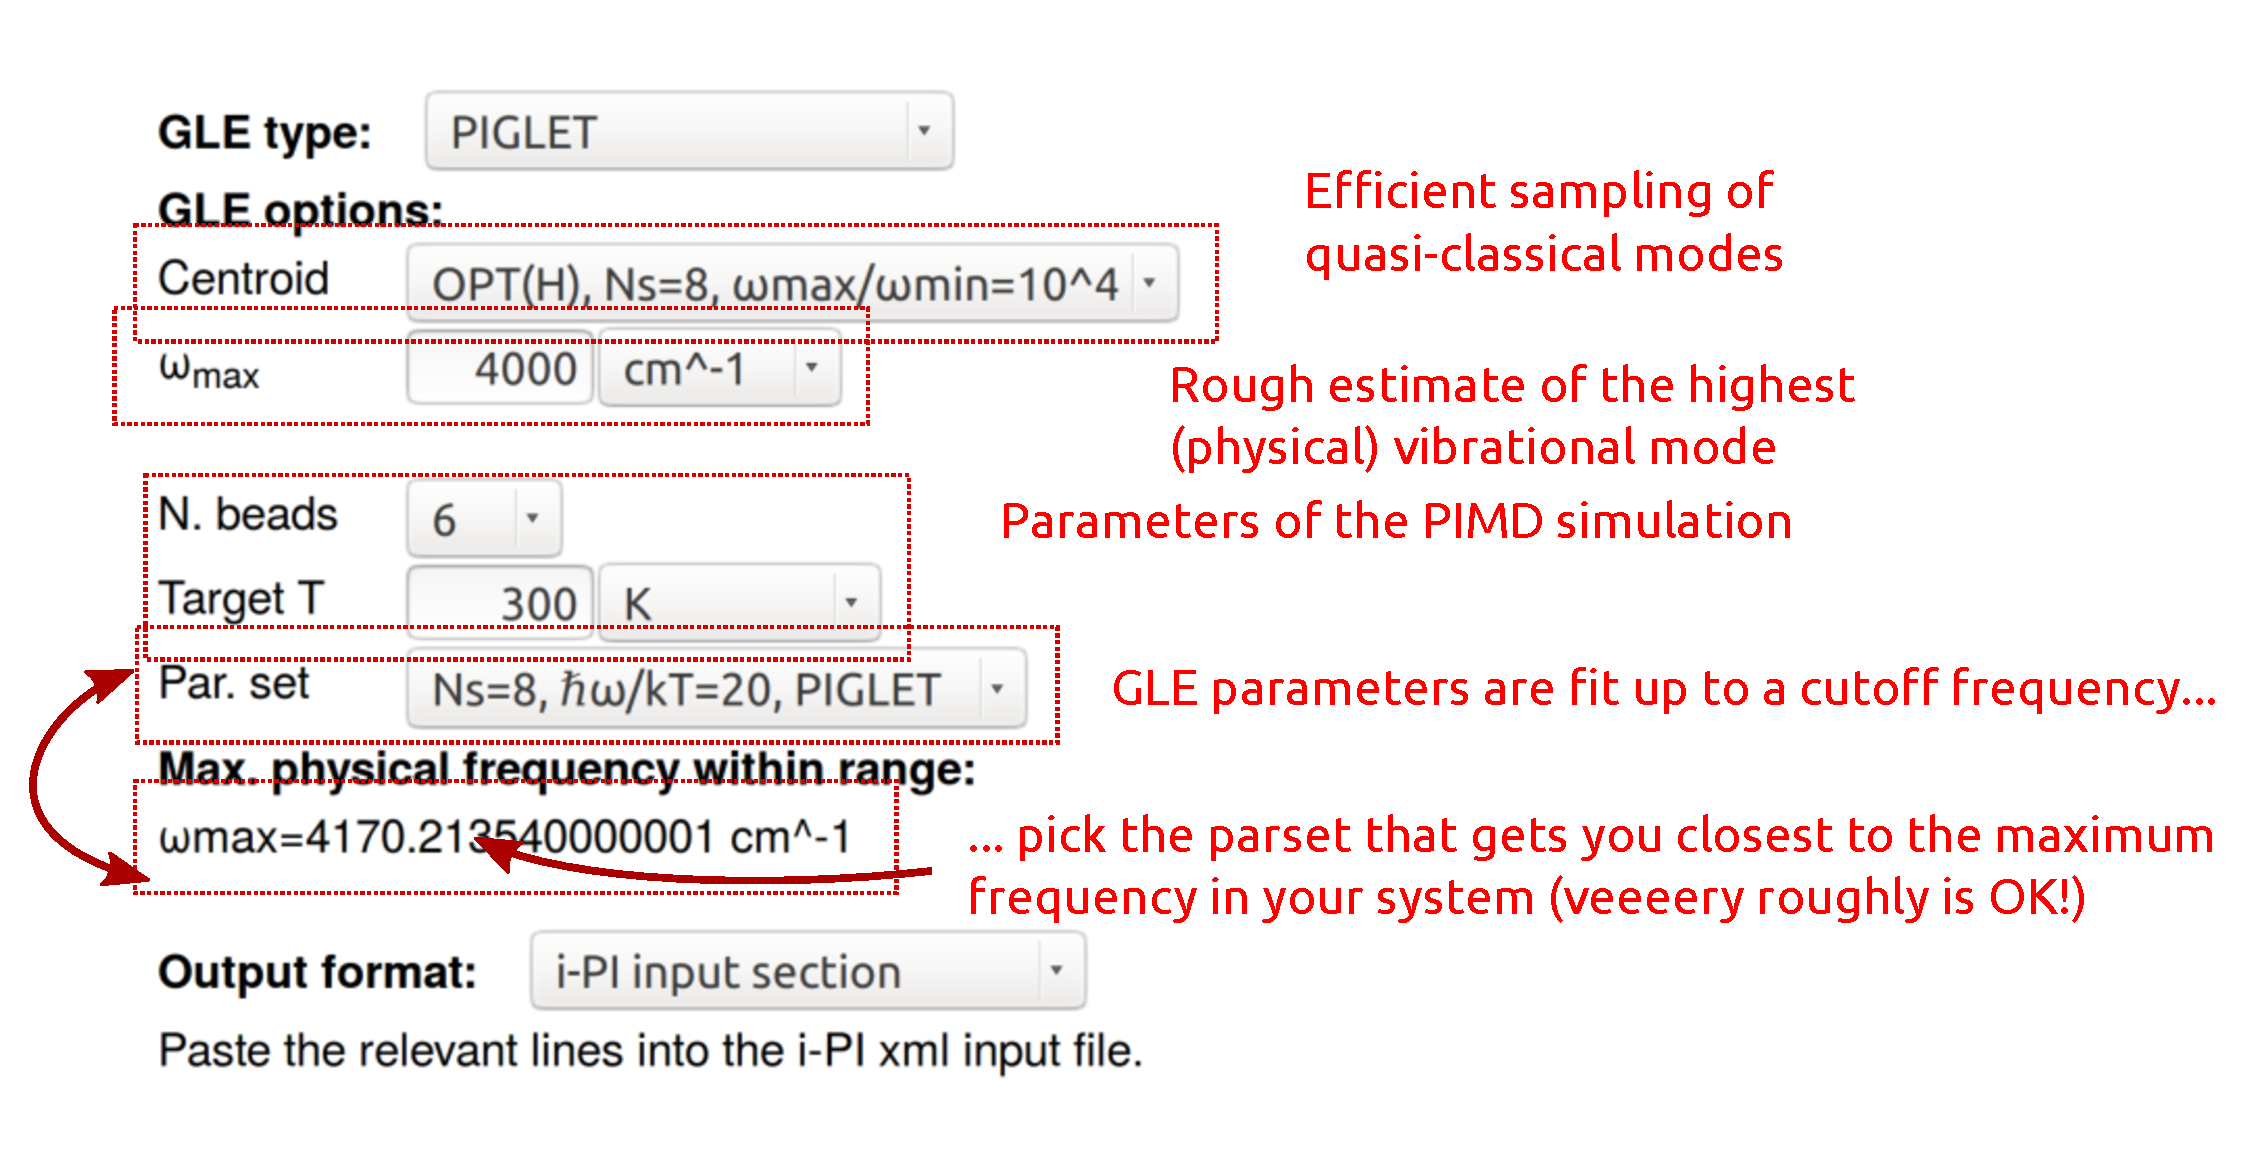
\includegraphics[width=1.0\textwidth]{gle4md.pdf}

\Question
Run your simulation -- the commands are pretty much the same as what you 
used in Exercise~\ref{basic}.  Compute the mean quantum and kinetic energy,
and compare them with the results you had from conventional PIMD. 

\Question 
Look also at the temperature of the ring polymer system. Remember: this temperature
is only an indication of the (classical) sampling of the ring-polymer Hamiltonian
and has no relation with the kinetic energy of the system. You will see that the mean
temperature differs from the one specified in \lstinxml$<ensemble>$. This is 
an indication of the out-of-equilibrium nature of PIGLET, and is perfectly normal --
nothing to worry about!

\Question Look also at the radial distribution functions. Consider that sampling 
time is also an issue: from these short simulations one cannot really 
make conclusive statements on the convergence of different techniques.

\end{Exercise}

\begin{Exercise}[label={npt},title={Variable-cell sampling}]

Let's now try to use the constant-pressure sampling features of i-PI to 
perform (colored-noise) path integral dynamics of water at high temperature
and GPa pressure. Note that the most interesting physics in these conditions
relates to high rates of self-ionization, that is observed in classical ab 
initio simulations~\cite{schw+01prl}, and is much enhanced by quantum 
effects~\cite{ceri+14cpc}. Unfortunately, in this tutorial we can only use
a non-dissociable forcefield and so we will not be able to explore this
aspect. 

\Question A working example is provided in the input file \url{ex-3/npt.xml}, 
but don't run it just yet. What thermostat is being used? How many beads? 
Although one may think that at such a high temperature quantum effects will be 
mild, it is a good idea to use a PIGLET thermostat just to be sure. 
Generate input parameters from \url{http://gle4md.org/index.html?page=matrix},
adapting them to the thermodynamic conditions considered here, substitute
the \lstinxml$<thermostat>$ field and launch your simulation. \hints{Note
that the barostat (a kind of a Langevin piston~\cite{buss+09jcp}, adapted
to PIMD~\cite{ceri+14cpc}) contains a separate  \lstinxml$<thermostat>$.
You should not touch this, or at least make sure you keep a classical thermostat,
since the degrees of freedom of the cell cannot be thermostatted with a 
quantum GLE (why? think of how the GLE infers the fluctuations from the time
scale of oscillations, and how the time scale of the cell dynamics is an
arbitrary parameter).}

\Question Analyze the run by observing the convergence of the cell volume
to the equilibrium value, and check that the pressure does fluctuate around the
target value. You can also visualize the variable-cell trajectory in VMD.
\hints{You can visualize the simulation box with the TCL command }
\begin{lstlisting}[language=bash]
vmd > pbc box
\end{lstlisting}



\end{Exercise}

\begin{Exercise}[label={sc-all},title={Doing PIMD Like a Pro}]
As a final example (in folder \url{ex-4/}) we will combine all the bits and pieces, performing
a simulation of ice at 100K, combining two different techniques to speed up
the calculation. We will use a fourth-order Suzuki-Chin factorization of
the Boltzmann operator~\cite{suzu95pla,chin97pla}, combined with a finite-difference
integrator~\cite{kapi+16}. Ring-polymer contraction~\cite{mark-mano08jcp} 
can also be used, that speeds up simulations by evaluating long-range interactions 
on a reduced number of beads.
%, and can be combined with a multiple-time step 
%integrator~\cite{tuck+92jcp} to exploit the same length-scale separation in the
%real-time integrator. 
We will not cover here the theory behind these techniques, 
so if you are not familiar with it, you are encouraged to read up the relevant 
literature before embarking in this exercise.
 \hints{These  start to be serious simulations, and it will not be possible 
to converge them at any decent level with a few minutes on a laptop. 
You can let them run overnight and/or run them on a more powerful computer
if you want to familiarize yourself with the convergence behavior of these 
accelerated PI methods.}

\Question Start by running the Suzuki-Chin simulation, that is
\begin{lstlisting}[language=bash]
$ i-pi highorder.xml &> log.ipi &
$ lmp_serial < in.ice &> log.lammps &
\end{lstlisting}
While the simulation runs, look at the input file. You'll notice
that we are outputting four more properties: 
\lstinxml$kinetic_opsc, kinetic_tdsc, potential_opsc, potential_tdsc$. These
are the `thermodynamic' and `operator' versions of the Suzuki-Chin estimators
for kinetic and potential energy. Note that -- contrary to the Trotter case --
the thermodynamic estimators are well-behaved when the number of beads is 
increased. You should see that after a few steps both the Td and the Op 
versions converge to very similar values, and that they are both significantly
different from the conventional estimators (that do not correspond to any
physical observable when sampling a fourth-order Hamiltonian, and are output
only for didactic purposes). \hints{Remember, when you compute averages, that 
you'll have to discard the (rather long) equilibration part, and that you should
use the columns that correspond to the S-C estimators.}

\Question Compute radial distribution functions. 
When inspecting trajectories,  remember that in SC path integrals you can 
evaluate structural observables by analyzing the even beads from the trajectory,
and ignoring the odd ones. You can try to compute RDFs for even and odd beads
separately, and verify that the two subsets sample different ensembles. 

\Question Finally, try to run the input file that also uses RPC
\begin{lstlisting}[language=bash]
$ i-pi ultimate.xml &> log.ipi &
$ lmp_serial < in.ice_long &> log.lammps &
$ lmp_serial < in.ice_short &> log.lammps &
\end{lstlisting}%$
Try to follow the complex simulation set up. If you are familiar with the structure
of LAMMPS input files, you'll notice that \url{in.ice_long} computes only
Lennard-Jones and Coulomb terms, while bonded terms contain dummy values.
Conversely, \url{in.ice_short} only computes the bonded (stretch and bend)
interactions. These two LAMMPS instances connect to two separate \lstinxml$<ffsocket>$
objects, that provide evaluators for the short and long-range components of
the force. Now, within the description of the \lstinxml$<system>$, you will
find the setup of the physical interactions, as they will be used by the 
integrator:
\begin{lstlisting}[language=xml]
 <forces>
   <force forcefield="lammps.long" nbeads="8"></force>
   <force forcefield="lammps.short" ></force>
 </forces>
\end{lstlisting}
This specifies that long-range forces should be 
%applied in the outer loop of a MTS scheme, and should be 
computed on a contracted ring polymer with only eight beads. Conversely, 
the short-range component should be computed
%in the second level of the MTS integrator, and should be computed 
on the default (total) number of beads, as specified in the \lstinxml$<initialize>$
section. 
%The definition of the force splitting is complemented by further
%parameters in the \lstinxml$<dynamics>$ section: the timestep refers to the
%total (outer) time, and the \lstinxml$<nmts>$ field specifies how many 
%iterations should be performed at every level of the MTS integrator.
Now compare the results with what you obtained with the \url{highorder.xml} 
input. You should observe only small differences, although considerably fewer
long-range force evaluations have been used. 
\hints{For a cheap potential as the one we consider here, communication
overhead is dominant, and so the speed-up will not be very noticeable. Nevertheless,
this strategy can be very advantageous when the long-range part of the interaction
is time-consuming, such as in an ab initio simulation.}

\end{Exercise}

\bibliographystyle{unsrt}
\bibliography{biblio.bib}
\end{document}
